\section{Objectif}

%%%%%%%%%%%%%%%%%%%%%%%%%%%%%%%%%%%%%%%%%%%%%%%%%%%%%%%%%%%%%%%%%%%%%%%%%%%%%%%%
%% Scénario
%%%%%%%%%%%%%%%%%%%%%%%%%%%%%%%%%%%%%%%%%%%%%%%%%%%%%%%%%%%%%%%%%%%%%%%%%%%%%%%%
\begin{frame}{Un exemple (fictif mais réaliste !)}
  \begin{block}{Scénario}
  On est jeudi soir et l'étudiant Ronan demande de l'aide à l'un de ses
  professeurs pour corriger son support de présentation pour la soutenance
  \emph{Boost Your Code}.\\
  ~\\
  \emph{Comment Ronan doit-il faire pour rendre le support accessible à son
  professeur et ainsi permettre la collaboration ?}
  \end{block}
\end{frame}

%%%%%%%%%%%%%%%%%%%%%%%%%%%%%%%%%%%%%%%%%%%%%%%%%%%%%%%%%%%%%%%%%%%%%%%%%%%%%%%%
%% Solution
%%%%%%%%%%%%%%%%%%%%%%%%%%%%%%%%%%%%%%%%%%%%%%%%%%%%%%%%%%%%%%%%%%%%%%%%%%%%%%%%
\begin{frame}{SVN}
\begin{columns}
  \begin{column}{.5\textwidth}
  SVN :
  \begin{itemize}
    \item Logiciel de gestion de versions
    \item Stocke un ensemble de fichiers en conservant la chronologie des
    modifications 
  \end{itemize}~

  Pour notre scénario :
  \begin{itemize}
    \item Le support de présentation est sur un serveur (\textbf{centralisé}).
    \item Les modifications se font en deux temps (\textbf{différé}).
  \end{itemize}
  \end{column}

  \begin{column}{.45\textwidth}
  \begin{figure}
    \center
    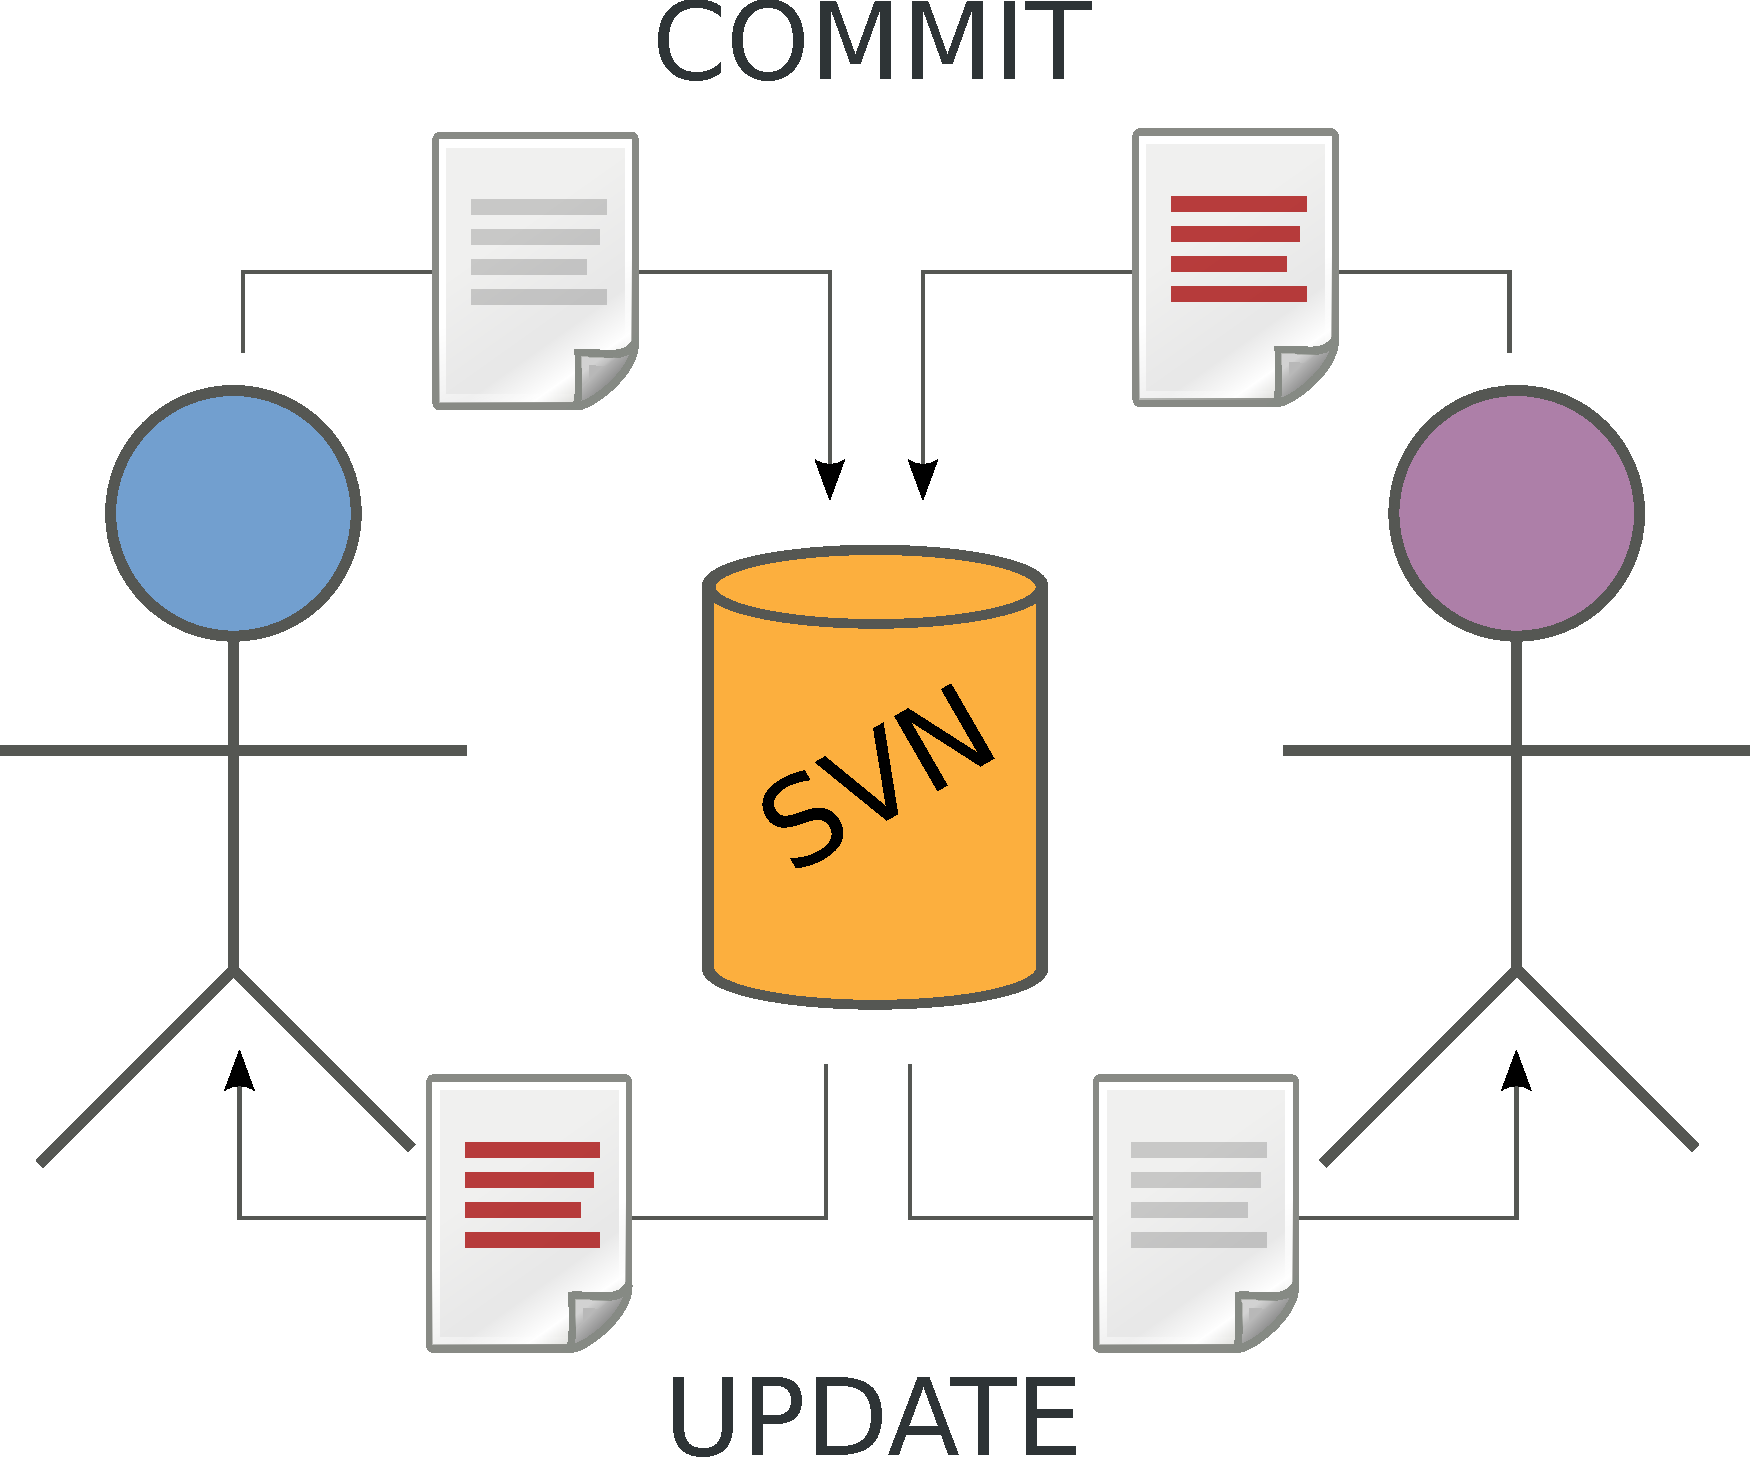
\includegraphics[width=.9\textwidth]{includes/svn.pdf}
    \caption{Solution SVN}
  \end{figure}
  \end{column}
\end{columns}
\end{frame}

\begin{frame}{Git}
\begin{columns}
  \begin{column}{.55\textwidth}
  Git :
  \begin{itemize}
    \item Logiciel de gestion de versions
    \item Système décentralisé
  \end{itemize}~

  Pour notre scénario :
  \begin{itemize}
    \item Chaque collaborateur a une copie du support de présentation
    (\textbf{distribué}).
    \item Les modifications se font en deux temps (\textbf{différé}).
  \end{itemize}
  \end{column}

  \begin{column}{.4\textwidth}
  \begin{figure}
    \center
    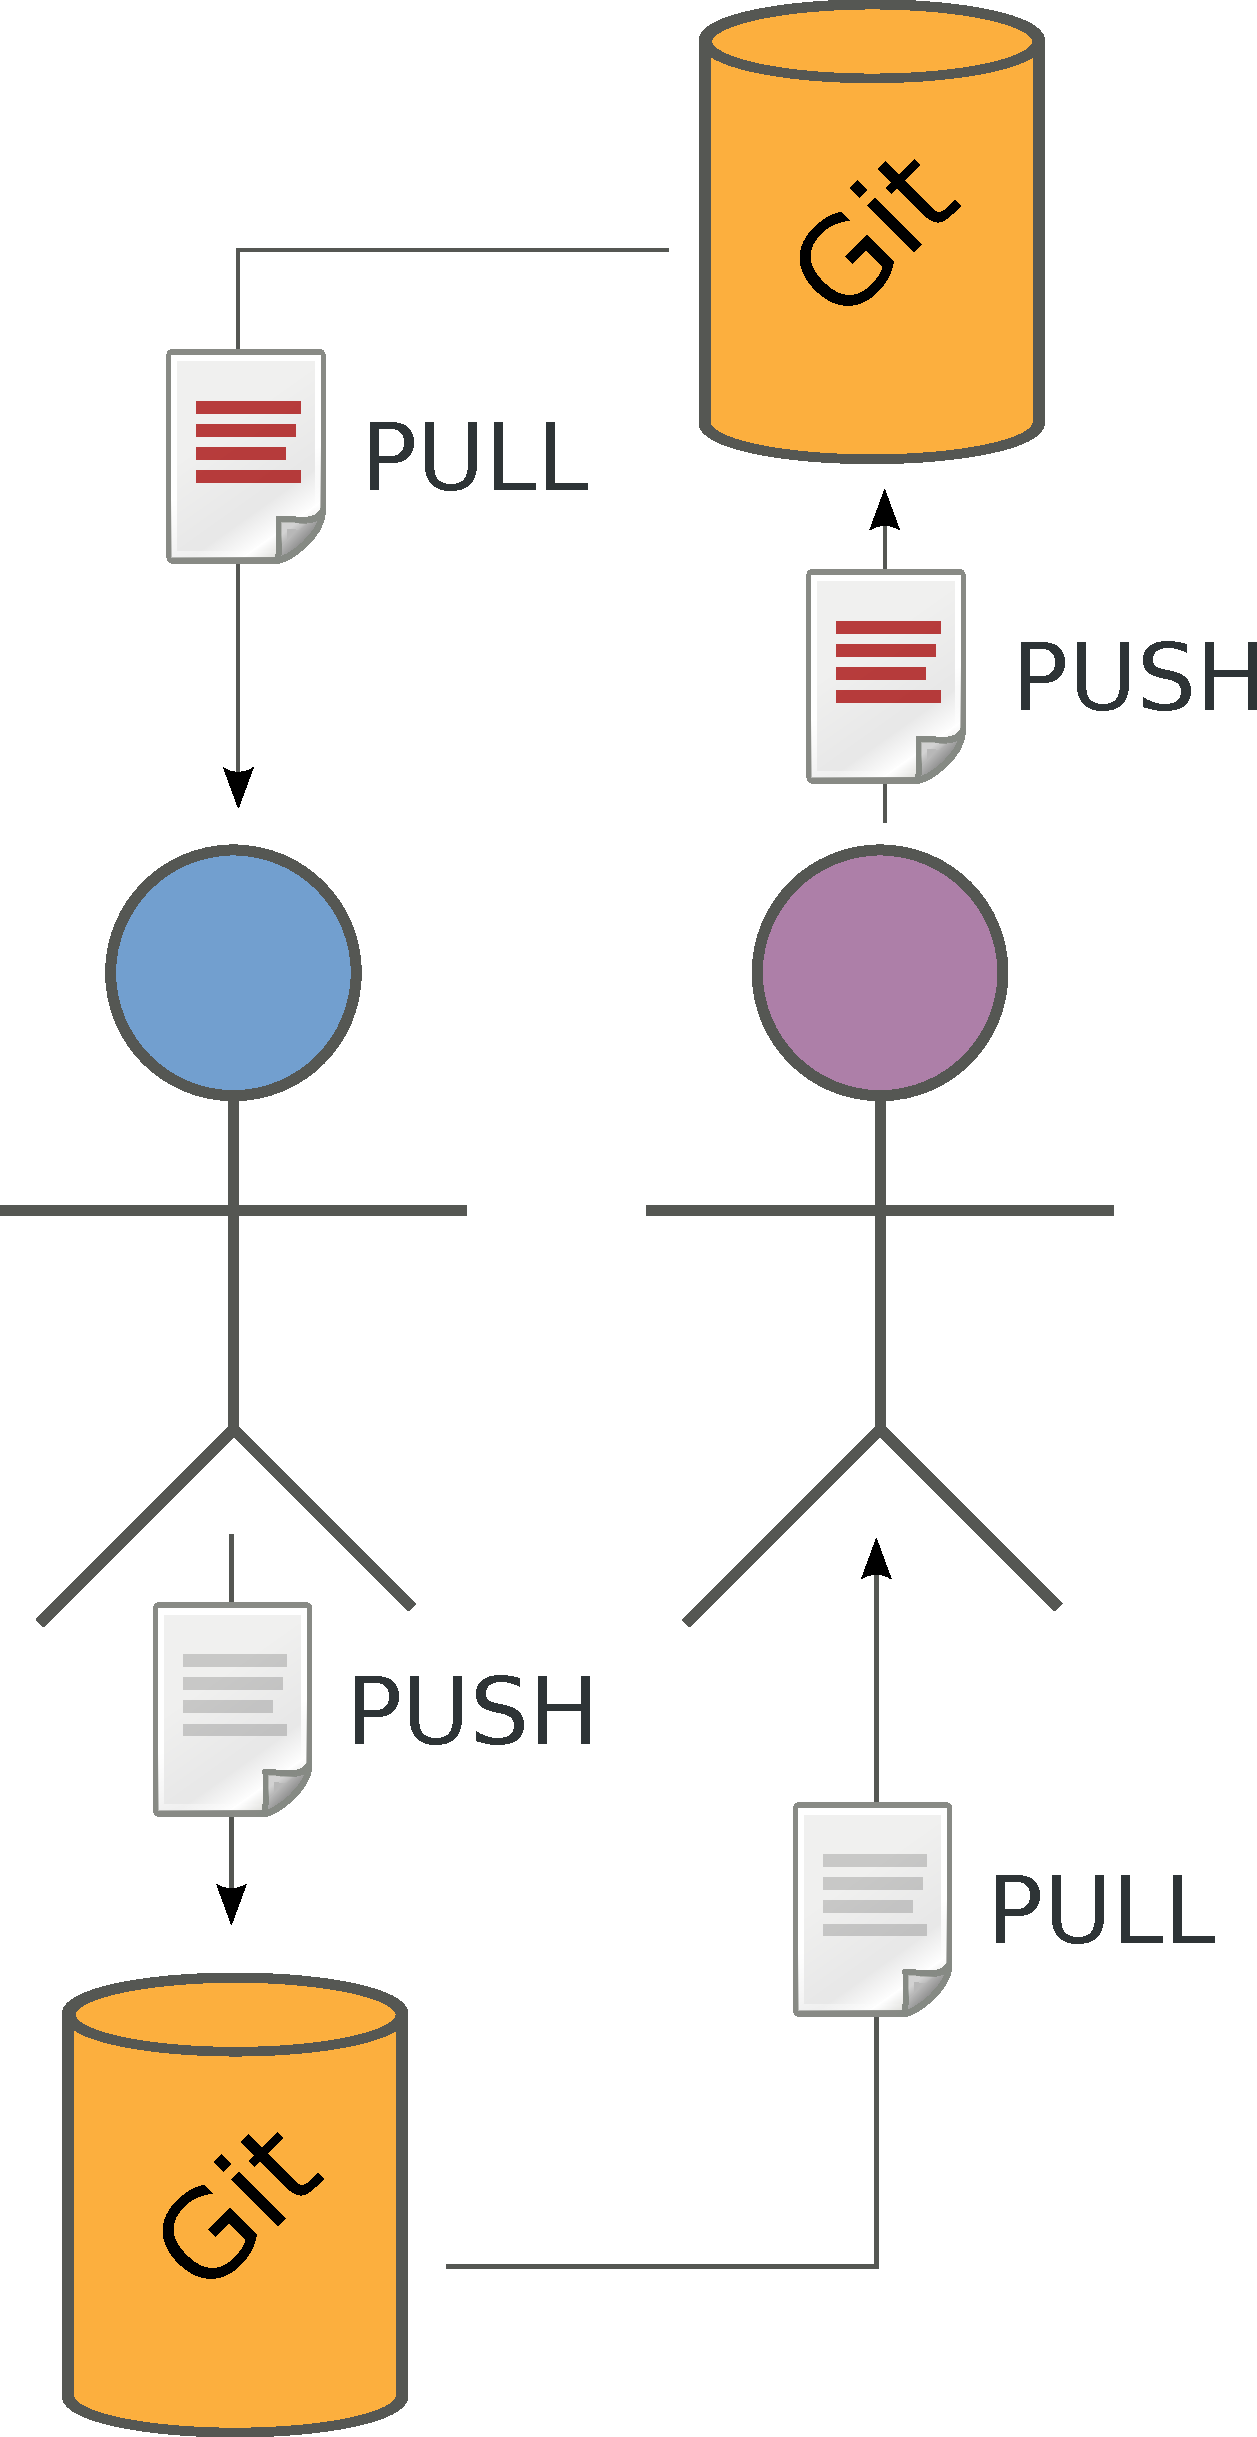
\includegraphics[height=.7\textheight]{includes/git.pdf}
    \caption{Solution Git}
  \end{figure}
  \end{column}
\end{columns}
\end{frame}

\begin{frame}{Google Docs}
\begin{columns}
  \begin{column}{.5\textwidth}
  Google Docs :
  \begin{itemize}
    \item Plateforme pour le travail collaboratif en ligne
    \item Permet l'édition de documents Word, Excel et PowerPoint
  \end{itemize}~

  Pour notre scénario :
  \begin{itemize}
    \item Le support de présentation est sur un serveur (\textbf{centralisé}).
    \item Les modifications se font en instantané (\textbf{temps réel}).
  \end{itemize}
  \end{column}

  \begin{column}{.45\textwidth}
  \begin{figure}
    \center
    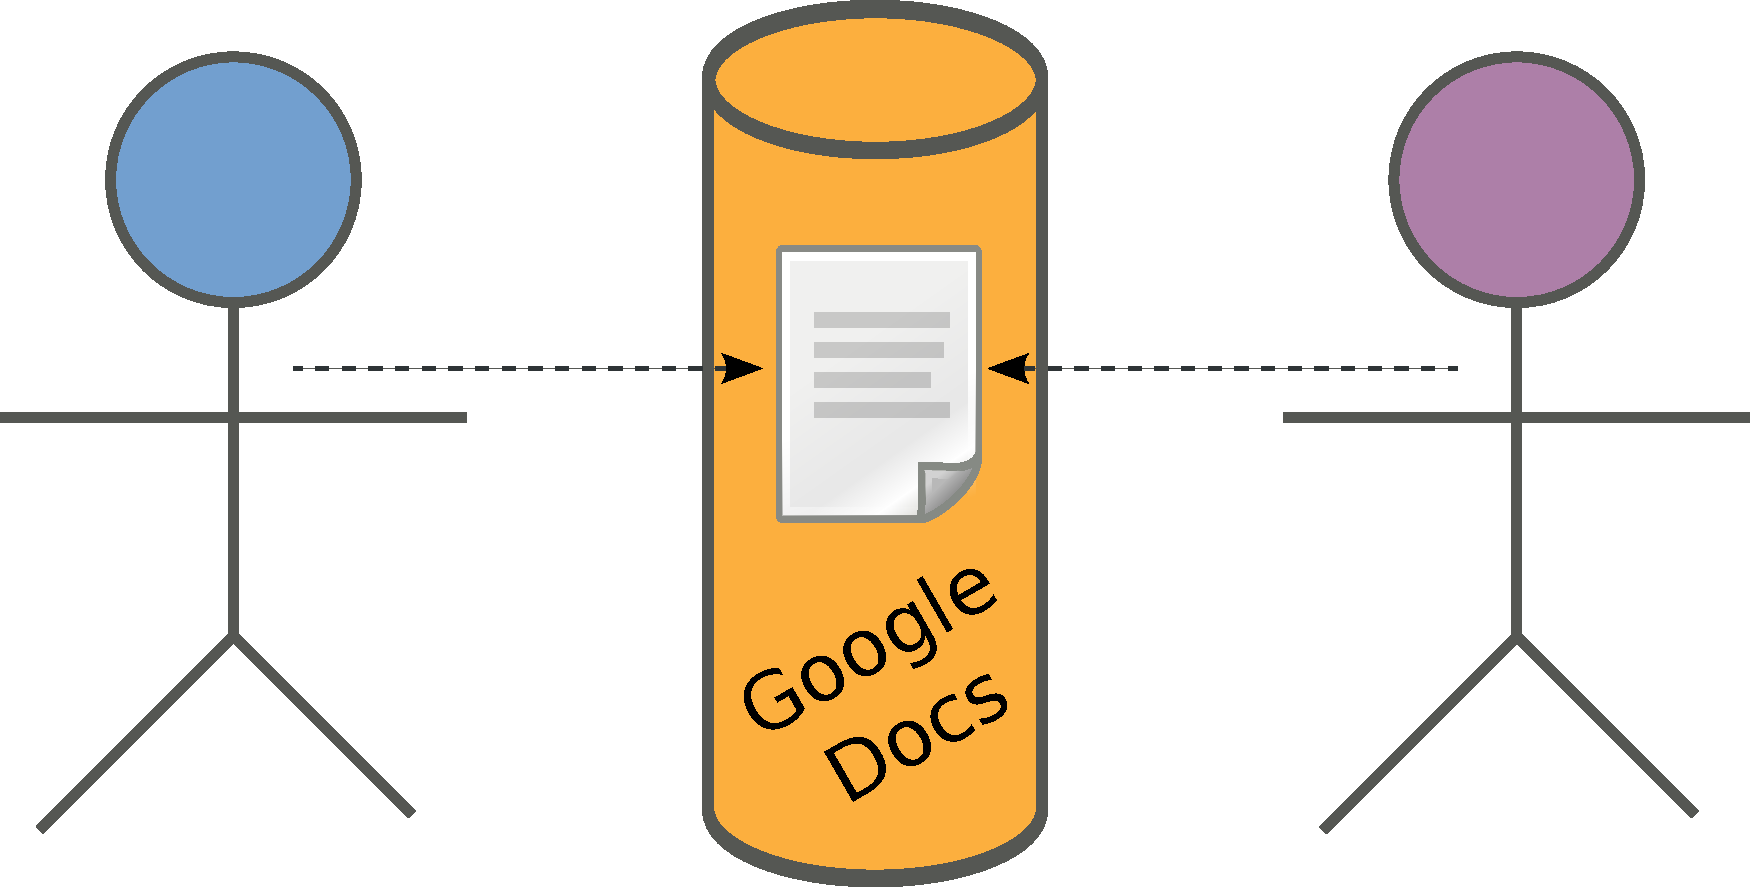
\includegraphics[width=.9\textwidth]{includes/gdocs.pdf}
    \caption{Solution Google Docs}
  \end{figure}
  \end{column}
\end{columns}
\end{frame}

\begin{frame}{Objectif}
  \begin{figure}
    \center
    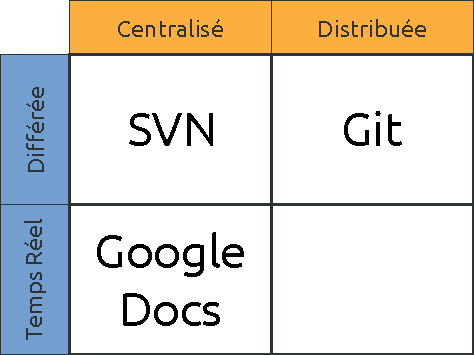
\includegraphics[width=.7\textwidth]{includes/tab1.pdf}
  \end{figure}
\end{frame}

\begin{frame}{Objectif}
  \begin{figure}
    \center
    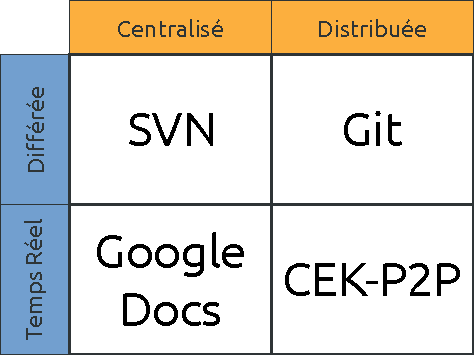
\includegraphics[width=.7\textwidth]{includes/tab2.pdf}
  \end{figure}
\end{frame}

\begin{frame}{Solution : \emph{CEK-P2P}}
  \begin{figure}
    \center
    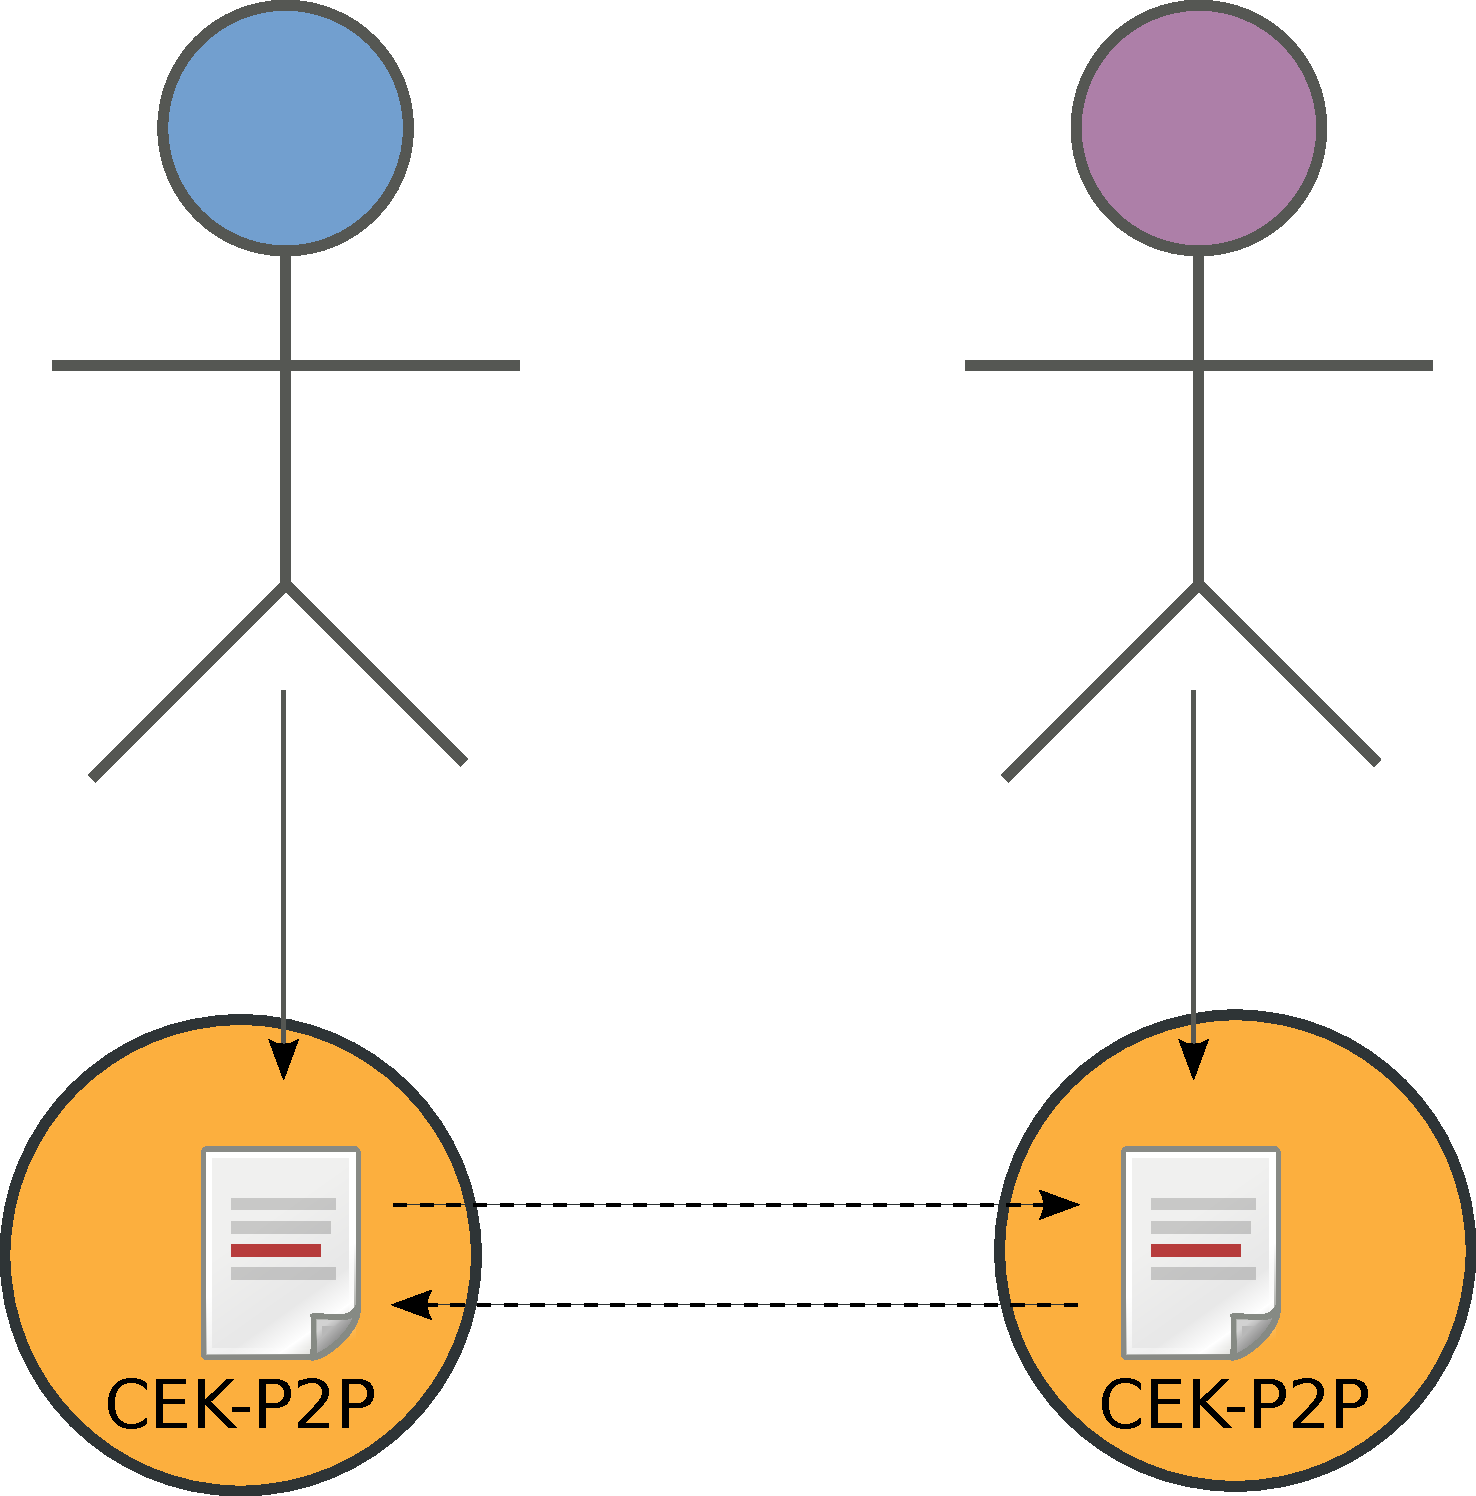
\includegraphics[width=.5\textwidth]{includes/cekp2p.pdf}
    \caption{Solution \emph{CEK-P2P}}
  \end{figure}
\end{frame}

\begin{frame}{Solution : \emph{CEK-P2P}}
  \begin{figure}
    \center
    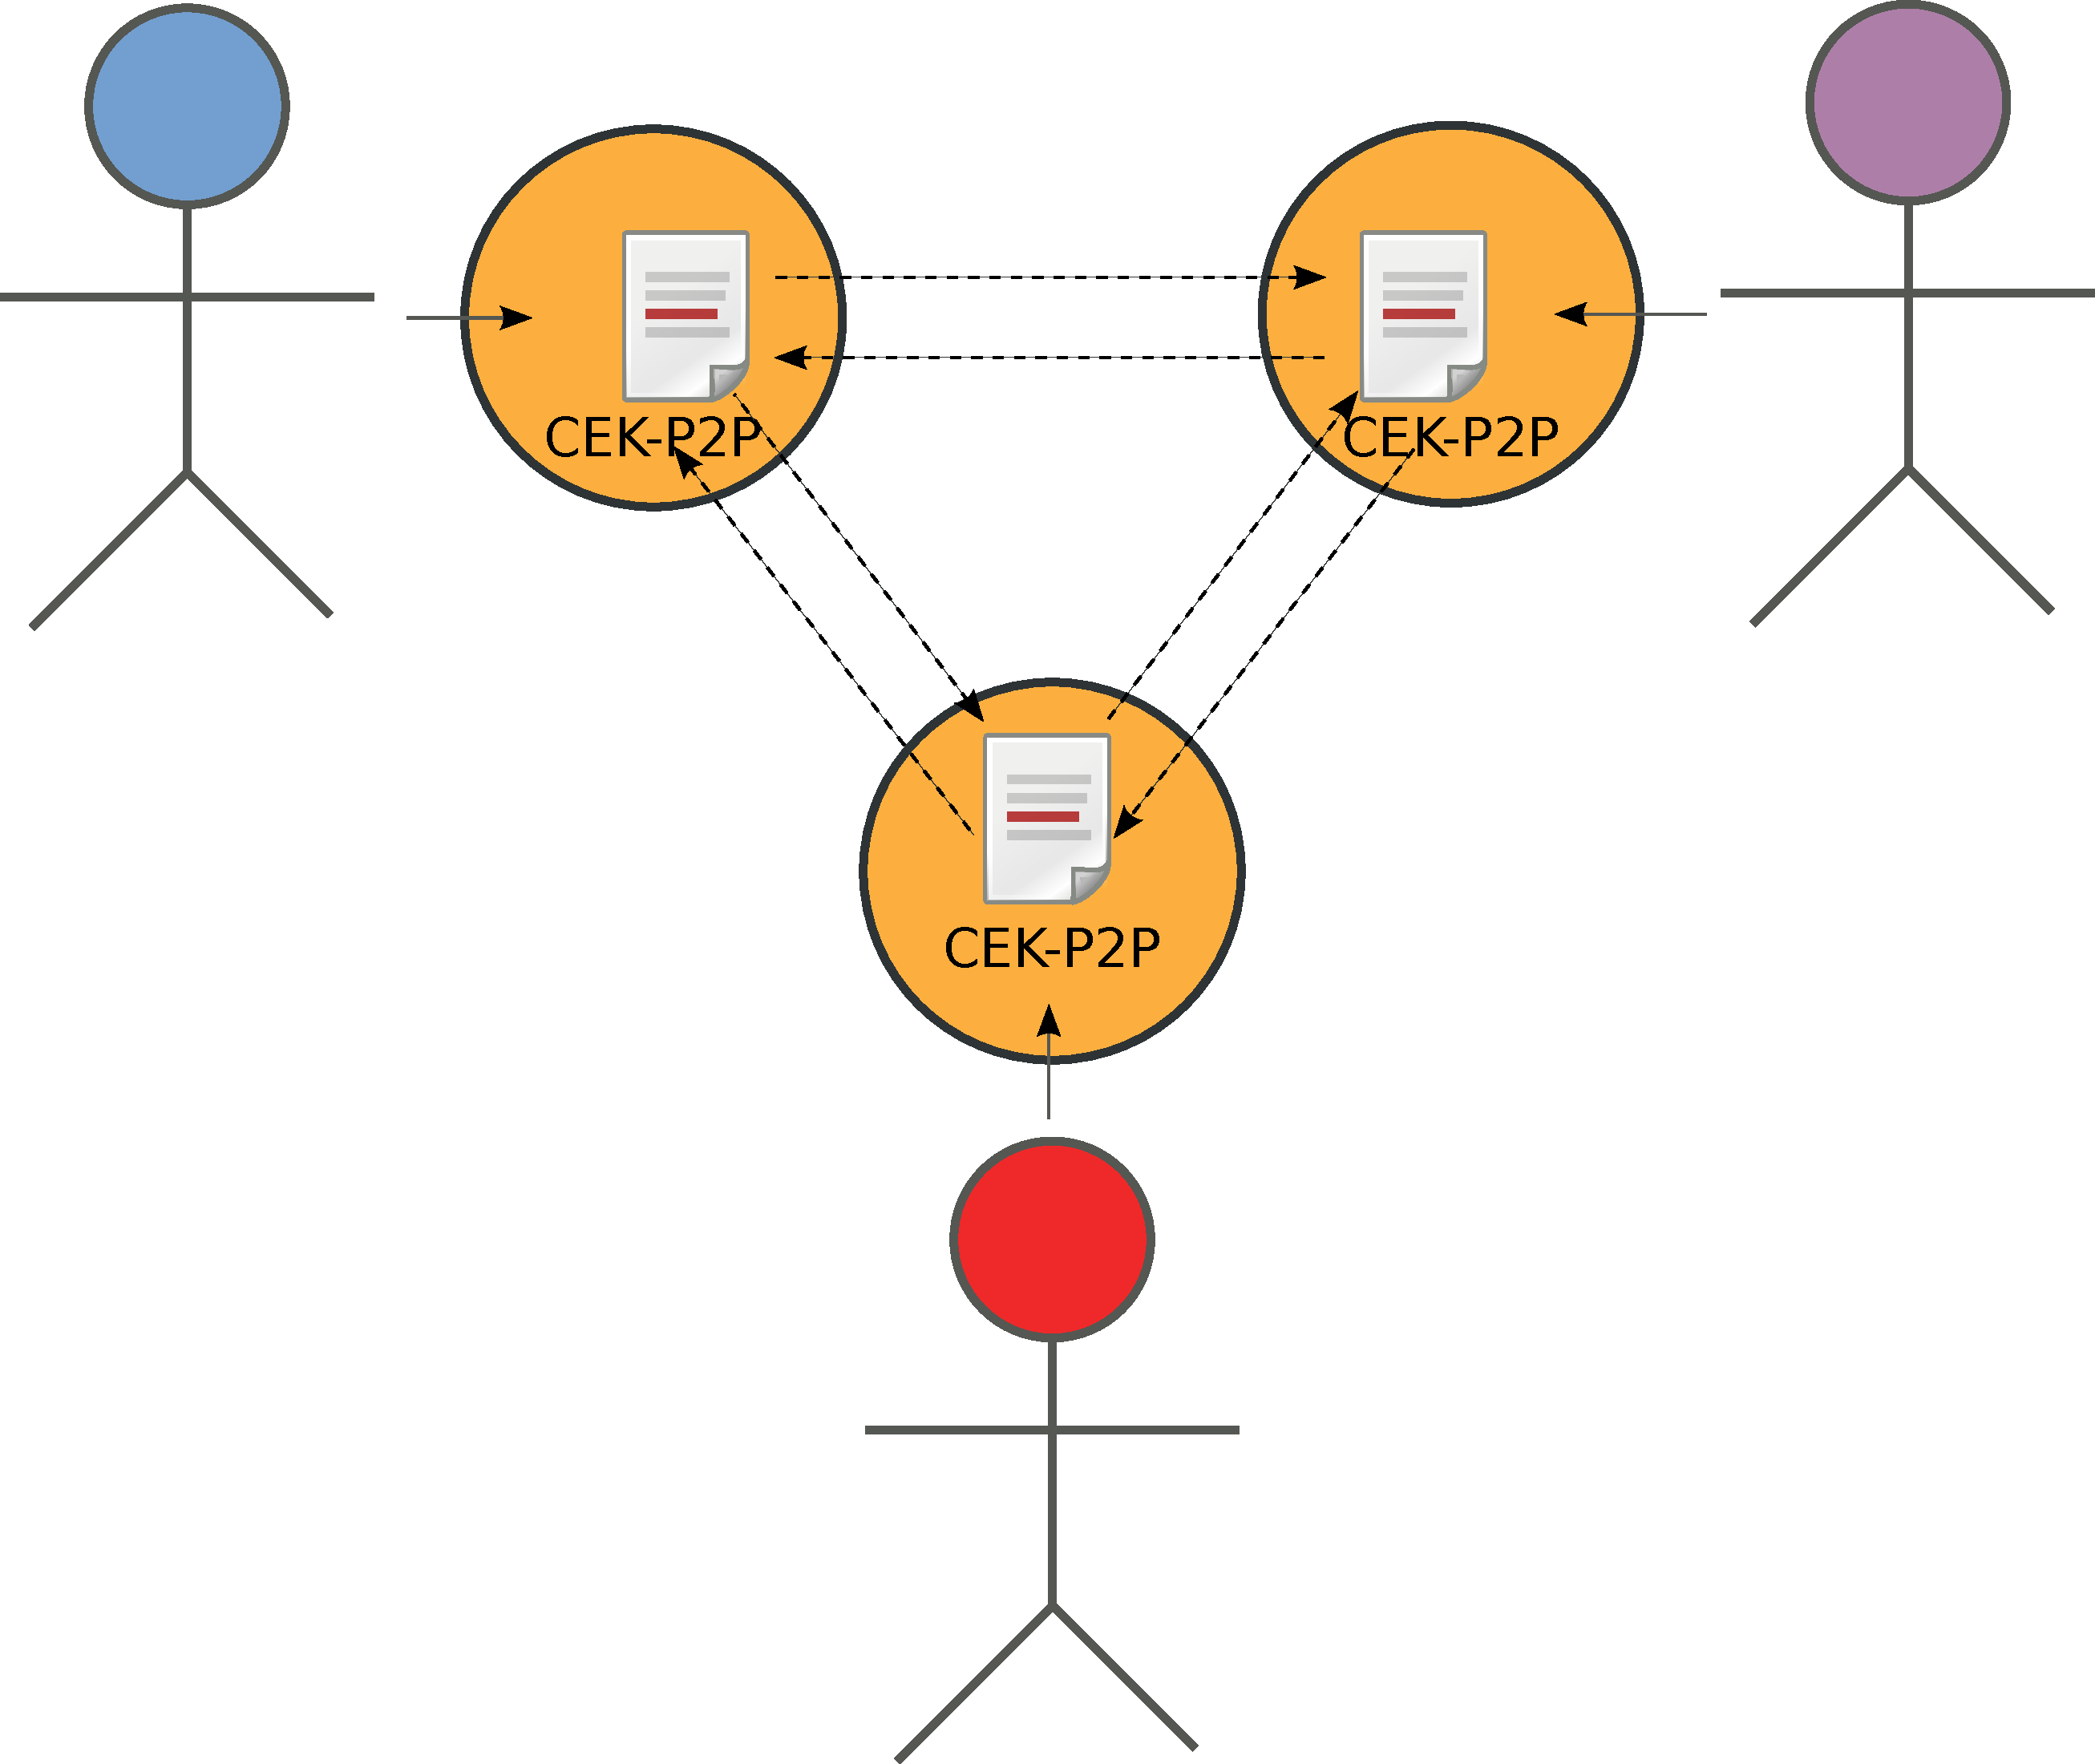
\includegraphics[width=.5\textwidth]{includes/cekp2p3perso.pdf}
    \caption{Solution \emph{CEK-P2P}}
  \end{figure}
\end{frame}

\begin{frame}{Le noyau : spécification}
\begin{itemize}
  \item Éditer plusieurs formats de documents : PowerPoint, Code Java, Sondage
  Doodle, \LaTeX, \ldots 
    \begin{itemize}
    \item[$\Rightarrow$] Méta-modèle de documents pour définir leur structure
    et leur édition
    \end{itemize}
  \item Particper au réseau Pair à Pair
    \begin{itemize}
    \item[$\Rightarrow$] Envoi et réception de messages
    \end{itemize}
  \item Envelopper des éditeurs existants
    \begin{itemize}
    \item[$\Rightarrow$] Architecture Modèle (Document) -- Vue (Éditeur) --
    Présentation (Intéraction)
    \end{itemize}
\end{itemize}
\end{frame}

